% =========================================================================
% AI-2 — Atividade de Orientação Individual (article format, Overleaf-ready)
% Distilling Tabular Foundation Models Beyond Classification
%
% Source of truth: paper/draft.md (audited twice: numeric review 8d7a64a,
% code review 8388abf). Every number traces to a versioned artifact in the
% repository — paths kept as LaTeX comments throughout.
% Compile: pdflatex -> bibtex -> pdflatex x2 (Overleaf default works).
% =========================================================================
\documentclass[11pt]{article}

\usepackage[utf8]{inputenc}
\usepackage[T1]{fontenc}
\usepackage[english]{babel}
\usepackage[margin=2.5cm]{geometry}
\usepackage{graphicx}
\usepackage{booktabs}
\usepackage{amsmath,amssymb}
\usepackage{textcomp}
\usepackage{microtype}
\usepackage[numbers,sort&compress]{natbib}
\usepackage[colorlinks=true,linkcolor=blue!60!black,citecolor=blue!60!black,urlcolor=blue!60!black]{hyperref}

\newcommand{\us}{\textmu s}

\title{\textbf{Distilling Tabular Foundation Models Beyond Classification:\\
Distributional Regression and the Distill/Compress/Cache Pareto Frontier}}

\author{João Gabriel de Araújo Vasconcelos\\
  \small Centro de Informática, Universidade Federal de Pernambuco\\
  \small \texttt{jgav@cin.ufpe.br}
  \and
  Germano Crispim Vasconcelos\\
  \small Centro de Informática, Universidade Federal de Pernambuco\\
  \small \texttt{[advisor email]}}
\date{Atividade de Orientação Individual --- July 2026}

\begin{document}
\maketitle

\begin{abstract}
Tabular foundation models now lead predictive accuracy: in our companion
benchmark of 14 models across 18 OpenML datasets, TabFM (Google, 2026) ranks
first in binary classification, multiclass, and regression, with TabPFN v2.5
a consistent second. This leadership carries an extreme cost: in-context
inference runs at 7.4--43\,ms/row --- four to five orders of magnitude slower
than gradient-boosted trees (0.33\,\us/row). Prior work distills tabular
foundation models for \emph{classification}; we study \emph{regression},
where the teacher's output is a predictive \textbf{distribution}. Across 20
datasets we find: (1) \textbf{point} distillation fails at realistic pool
sizes regardless of teacher strength --- a robust negative replicated with
two teachers; (2) \textbf{distributional} distillation --- transferring the
teacher's quantile curves into a multi-quantile student --- retains a median
19\% and up to 100\%+ of the teacher's CRPS advantage (positive in 16/20
datasets, including one born-again case where the student surpasses its
teacher; one-sided sign test $p = 0.006$, Wilcoxon $p = 0.045$, Bayesian
$P(\mathrm{ret}>0) = 0.70$) at microsecond latency, making the distilled
student the only sub-millisecond distributional system on our three-strategy
Pareto frontier (distill vs.\ context compression vs.\ ensemble reduction);
(3) out-of-fold labeling matters for the student's \textbf{calibration}, not
its accuracy --- a deconfounded refinement of prior classification findings;
and (4) failures are diagnosable, yielding a practical decision rule: try
target transforms and a strong native student first, and distill when a
genuine teacher edge persists --- cheaply verifiable via OOF labeling. All
experiments are pre-registered, seed-controlled, and publicly reproducible
on a single 16\,GB GPU.
\end{abstract}

\section{Introduction}

For a decade, the practical advice for tabular prediction was stable:
gradient-boosted decision trees (GBDTs) win
\citep{grinsztajn2022,mcelfresh2023}. The 2024--2026 generation of tabular
deep learning and, decisively, of tabular foundation models (TFMs) has
overturned the accuracy half of that advice. In a uniform-protocol benchmark
we ran of 14 models $\times$ 18 OpenML datasets (nested cross-validation,
per-family preprocessing, equal tuning budgets), the zero-shot TabFM ranks
first on all three task types and is the single best model on 13 of 18
datasets; TabPFN v2.5 \citep{hollmann2025,priorlabs2025} is the consistent
runner-up.
% notebooks/TABELA_RESULTADOS.md; results/aggregated/test_results.csv

The cost half of the advice, however, has inverted rather than disappeared.
In-context learners carry their training set as context at prediction time:
we measure 7{,}416\,\us/row for TabPFN and 43{,}262\,\us/row for TabFM on
the \texttt{adult} dataset, against 0.33\,\us/row for tuned XGBoost --- a
factor of 22{,}000$\times$ and 131{,}000$\times$ respectively.
% results/latency/latency_adult.csv
A leave-one-dataset-out policy analysis over the same benchmark shows that
``use the foundation model by default'' has median normalized regret 0.000
--- the \emph{only} obstacle to that policy is serving cost.
% results/aggregated/lodo_validation_14.csv

Knowledge distillation \citep{bucila2006,hinton2015} is the natural attack
on that obstacle, and recent work has established it for tabular
\textbf{classification} \citep{pocketfm2026}. Regression, however, is not
classification with a continuous label: modern TFMs output a full
\emph{predictive distribution} (TabPFN's bar-distribution head), and the
value of that distribution --- calibrated uncertainty at prediction time ---
is precisely what a point-label student cannot learn from raw data alone.
This paper asks what distillation can and cannot transfer in tabular
regression, at what serving cost, and under which verifiable conditions.

\paragraph{Contributions.}
\begin{enumerate}
  \item \textbf{A robust negative:} point distillation of TFMs fails as a
    rule at realistic pool sizes (soft targets beat the hard-label control
    in only 4/20 datasets), replicated with two teachers of very different
    strength, with a pool-size sweep showing the residual gain is a
    small-data phenomenon on some datasets only.
  \item \textbf{A positive on the open axis:} distributional distillation
    via quantile-curve transfer is positive in 16/20 datasets --- the
    complete eligible CTR23 pool under a rule fixed before any results ---
    with median retention 19\%, maximum above 100\% (a born-again student),
    and agreement across instruments (sign test $p = 0.006$; Wilcoxon
    $p = 0.045$; Bayesian signed-rank $P(\mathrm{retention}>0) = 0.70$ at
    ROPE $\pm 0.05$), at microsecond latency.
  \item \textbf{The first three-strategy Pareto frontier} for TFM serving
    in regression --- distillation vs.\ context compression vs.\ ensemble
    reduction --- measured end-to-end on the same hold-outs; below
    ${\sim}250$\,\us/row (up to ${\sim}1.3$\,ms/row on our largest dataset)
    the distilled student is the only distributional option, and
    side-findings show ensemble reduction is underrated (1 member $\approx$
    8 at 1/7 the latency) while the last context doubling is grossly
    overpriced on 16\,GB GPUs.
  \item \textbf{A deconfounded account of why out-of-fold labeling matters
    in regression:} in-sample teacher labels do not hurt student accuracy
    or CRPS --- they erode interval \emph{coverage} ($-0.5$ to $-5.1$~p.p.\
    at fixed context size), i.e., the teacher's in-context overconfidence
    transfers to the student.
  \item \textbf{A practical decision rule} distilled (pun intended) from
    two refuted hypotheses: before distilling, apply cheap target
    transforms and try a strong native quantile student; distill when a
    genuine teacher edge survives both --- verifiable with one inexpensive
    OOF pass.
\end{enumerate}

\section{Related Work}

\paragraph{Tabular foundation models.} TabPFN v2/v2.5
\citep{hollmann2025,priorlabs2025} established prior-fitted in-context
learning for tabular data; TabICL \citep{tabicl2025}, TabFlex
\citep{tabflex2025} and MotherNet \citep{mothernet2023} explore faster or
amortized variants; TabFM \citep{tabfm2026} is an independent implementation
of the paradigm with a hybrid column-attention/row-compression architecture,
released with weights but --- as of this writing --- no peer-reviewed
reference (we cite the official blog and model card, and pin the version).
Our companion benchmark provides the neutral evidence of the accuracy
leadership and the latency inversion that motivate this paper.

\paragraph{Distilling TFMs.} Pocket FM \citep{pocketfm2026} distills
classification TFMs (TabICLv2, TabPFNv2.6, LimiX, Orion-MSP) into
XGBoost/CatBoost/MLP students on 153 datasets, retaining 96.5\% of teacher
AUC at 38--860$\times$ speedups, and establishes stratified out-of-fold
labeling as necessary; a companion paper extends the analysis to clinical
data \citep{pocketfmhealth2026}. Prior Labs ships a closed-source
distillation engine for TabPFN-2.5 \citep{priorlabs2025}. TabDistill
\citep{tabdistill2025} targets few-shot MLP students; another line distills
TFMs into GAMs for interpretability \citep{tfmgam2026}. None of these
addresses regression, distributional outputs, or a cross-strategy serving
frontier --- the axes of this paper. The classical lineage (model
compression via soft labels \citep{bucila2006,hinton2015}; born-again trees
\citep{breiman1996,vidal2020,frosst2017}) supplies the mechanics we adapt
to quantile curves.

\paragraph{Acceleration without distillation.} TACO \citep{taco2026}
compresses the in-context set to ${\sim}1\%$ with large speedups; CRUMB
\citep{crumb2026} selects a compact context via MMD for efficient PFN
inference without retraining --- a representative method of the
context-compression arm our frontier measures; MotherNet
\citep{mothernet2023} amortizes fitting into a hypernetwork that emits MLP
weights; TL-ANDI \citep{tlandi2026} combines locally distilled labels with
optimal-transport context selection for cross-task transfer (orthogonal
goal, no fast students, no distributional axis); simple engineering
(context truncation, ensemble reduction, KV-caching) is folklore. Our
frontier measures the engineering strategies head-to-head with distillation
on identical hold-outs. On OOF labeling specifically, the health-data
companion of Pocket FM \citep{pocketfmhealth2026} already establishes
stratified OOF for classification soft-labels; our contribution on that
axis is confined to what OOF protects in \emph{distributional regression}
--- calibration, not accuracy (\S\ref{sec:oof}).

\paragraph{Distributional regression.} Quantile regression with pinball
loss \citep{koenker1978}, CRPS as a proper scoring rule
\citep{gneiting2007}, and coverage/sharpness diagnostics are standard;
XGBoost $\geq$2.0 \citep{chen2016} supports native multi-quantile
objectives, which we use both as a hard-label control and as the student
body for curve transfer.

\section{Method}

\paragraph{Teachers.} TabPFN v2.5 is our distributional teacher (v2.5
rather than the newer TabPFN-3 \citep{tabpfn3-2026} for version-pinned
comparability with the companion benchmark and verified 16\,GB-GPU
operation; nothing in our method is version-specific): its native API
returns arbitrary quantiles of the predictive distribution, from which we
take a 19-level grid ($\tau = 0.05, \ldots, 0.95$). TabFM is a point-only
teacher --- we verify architecturally (its regression head decodes a single
scalar) and empirically (its 8-member ensemble spread yields CRPS 0.524
vs.\ the TabPFN teacher's 0.069 on \texttt{california\_housing}, with
16.3\% coverage at 80\% nominal) that no usable predictive distribution is
available from it.
% results/distillation/tabfm_spread.csv
Both teachers run with an 8-member inference ensemble and a 50k-row context
cap, matching the companion benchmark's policies (for TabFM, 8 members
measured accuracy-equivalent to the library default of 32 at $\tfrac14$ the
cost).

\paragraph{Out-of-fold labeling.} Teacher targets for every training row
come from a $K{=}5$ out-of-fold scheme: the teacher conditioned on 4/5 of
the pool labels the held fifth. Labels are cached once per (dataset,
teacher) and reused by all student variants.

\paragraph{Students and targets.} All students inherit the tuned
hyperparameters of the corresponding baseline from the companion benchmark
--- capacity is held fixed and only the target changes, isolating the
distillation effect.
\begin{itemize}
  \item \emph{XGBoost point}, trained on true labels (control), on the
    teacher's OOF mean (soft), or on a 0.8/0.2 mixture.
  \item \emph{XGBoost multi-quantile}: hard variant uses the native pinball
    objective on true labels; soft variant fits the 19 teacher quantile
    curves as a multi-output regression (crossing repaired by row-wise
    sorting).
  \item \emph{MLP-quantile}: the benchmark's MLP body with a 19-output
    head; pinball on labels (hard) or MSE on teacher curves (soft) ---
    symmetric with the XGBoost pair, to test whether the student family
    matters.
\end{itemize}

\paragraph{Metrics.} RMSE and MAE for point quality; CRPS estimated as
twice the mean pinball loss over the 19-level grid --- the standard grid
estimator in probabilistic-forecasting practice, which we validated against
the Gaussian closed form: it carries a near-constant multiplicative
overestimate of ${\sim}4$--5\%, so within-paper comparisons and retention
ratios are unaffected but absolute CRPS values should not be compared
across papers; PICP80/90 with interval widths for calibration; and a
normalized retention score,
\begin{equation}
  \mathrm{retention} \;=\;
  \frac{\mathrm{CRPS}_{\mathrm{hard}} - \mathrm{CRPS}_{\mathrm{soft}}}
       {\mathrm{CRPS}_{\mathrm{hard}} - \mathrm{CRPS}_{\mathrm{teacher}}},
\end{equation}
where 1 means the student recovers the teacher's entire edge over its own
hard-label control and negative values mean distillation hurt. Latency is
\us/row on the benchmark hold-out (median of 5 passes for students; single
timed pass for teachers, whose per-pass cost is minutes).

\paragraph{Pre-registration and conduct.} Hypotheses, gates, and decision
criteria were registered before execution; deviations are dated addenda;
negative results are reported with the same prominence as positives; and
one labeling erratum discovered mid-study (a config key pointing to the
wrong OpenML id) is documented with its full rectification trail --- the
accidental duplicate run it produced doubles as an exact end-to-end
reproducibility check of the pipeline.
% docs/desenho-experimental-destilacao.md; docs/errata-diamonds-kin8nm.md

\section{Experimental Setup}

Five regression datasets from the companion benchmark
(\texttt{wine\_quality}, \texttt{california\_housing},
\texttt{superconduct}, \texttt{kin8nm}, \texttt{year\_prediction}; pools
5.2k--80k) plus the complete eligible pool of fifteen from the OpenML-CTR23
suite \citep{fischer2023} under verified constraints (3k--100k rows; two
suite datasets excluded for target leakage discovered during verification
--- the target is a sum of features in \texttt{brazilian\_houses} and
\texttt{wave\_energy}; version-pinned dataset ids). Splits are identical to
the companion benchmark: a fixed 20\% hold-out (seed 42) that no selection
step ever observes; three student seeds throughout. Hardware: a single
RTX~5080 (16\,GB); VRAM ceilings are treated as measurements, not nuisances
(\S\ref{sec:frontier}).
% configs/datasets.yaml (regression_extension); scripts/extension_ctr23.py

\section{Results}

\subsection{Point distillation fails at scale --- with any teacher}
\label{sec:point}

Across all 20 datasets, the point student trained on teacher means beats
its hard-label control in only 4; with the far stronger TabFM teacher
(anchor gaps up to 4$\times$ larger, e.g.\ 0.031 vs.\ 0.008 RMSE on
\texttt{california\_housing}) the picture is unchanged --- only
california's two soft-target cells beat the hard-label control at all, with
best within-pipeline retention 0.11 (california/mixed); the remaining eight
cells are at or below the control. A pool-size sweep (caps 800/2k/8k) shows
a genuine small-data gain on \texttt{wine\_quality} ($\Delta = +0.026$ at
$n{=}800$) that vanishes by $n{=}2{,}000$ and does not replicate on
\texttt{california\_housing}; we report it as an observation with a
dataset-dependent moderator, not a general effect. Conclusion: at realistic
pool sizes, a tuned GBDT extracts as much point accuracy from the raw
labels as from the teacher's opinions of them.
% results/distillation/distill.csv, distill_cap*.csv, extension.csv

\subsection{Distributional distillation works --- where the teacher has an
edge}
\label{sec:dist}

Transferring the teacher's quantile curves changes the outcome. Over the
complete 20-dataset pool (Table~\ref{tab:retention}), CRPS-gap retention is
positive in 16 (median $+0.19$), topping at $+1.06$ (\texttt{pumadyn32nh}
--- a born-again student that surpasses its teacher), $+0.64$
(\texttt{california\_housing}), $+0.59$ (\texttt{abalone}), $+0.52$
(\texttt{fps\_benchmark}) and $+0.50$ (\texttt{cpu\_activity}). Both
frequentist instruments reject at the 5\% level (one-sided sign test
$p = 0.006$; Wilcoxon $p = 0.045$) and the Bayesian signed-rank
\citep{benavoli2017} places 0.70 posterior mass on positive retention at
ROPE $\pm 0.05$ (0.63--0.71 across ROPE 0.02--0.10). The four failures are
diagnosable and form the basis of \S\ref{sec:rule}'s decision rule:
\texttt{wine\_quality} --- where the teacher trails the tuned baseline on
RMSE (the axis of our pre-registered gate) and its small CRPS edge
($+0.04$) inverts under transfer --- and three price-scale, heavy-tailed
targets (\texttt{fifa}, \texttt{diamonds}, \texttt{health\_insurance})
where \S\ref{sec:rule} shows the teacher's apparent edge is largely
reproducible by a log transform.

Calibration accompanies the transfer --- and exceeds it. Reliability curves
(Fig.~\ref{fig:calibration}) show the distilled student closest to the
diagonal on both panels; on \texttt{california\_housing} it is better
calibrated than the hard control \emph{and} than its own teacher, whose
per-level quantile calibration is imperfect (S-shaped). Curve transfer plus
sorting acts as a calibration regularizer, not a mere copy.
% results/distillation/distill.csv + extension.csv;
% results/figures/calibration_distill.pdf

\begin{table}[t]
\centering
\caption{CRPS-gap retention of the distilled multi-quantile student over
all 20 datasets (mean of 3 seeds; teacher edge
$= \mathrm{CRPS}_{\mathrm{hard}} - \mathrm{CRPS}_{\mathrm{teacher}}$, in
target units). Positive in 16/20; median $+0.19$.
Source: \texttt{results/distillation/paper\_retention.csv}.}
\label{tab:retention}
\small
\begin{tabular}{llrr}
\toprule
Dataset & Source & Retention & Teacher edge \\
\midrule
pumadyn32nh            & CTR23 & $+1.057$ & 0.001 \\
california\_housing    & core  & $+0.644$ & 0.111 \\
abalone                & CTR23 & $+0.595$ & 0.095 \\
fps\_benchmark         & CTR23 & $+0.523$ & 0.152 \\
cpu\_activity          & CTR23 & $+0.500$ & 0.233 \\
cps88wages             & CTR23 & $+0.465$ & 0.345 \\
year\_prediction       & core  & $+0.419$ & 0.311 \\
superconduct           & core  & $+0.255$ & 0.006 \\
sarcos                 & CTR23 & $+0.225$ & 0.474 \\
kings\_county          & CTR23 & $+0.213$ & 7253.4 \\
grid\_stability        & CTR23 & $+0.170$ & 0.003 \\
kin8nm                 & core  & $+0.128$ & 0.030 \\
physiochemical\_protein& CTR23 & $+0.086$ & 0.573 \\
video\_transcoding     & CTR23 & $+0.086$ & 0.092 \\
space\_ga              & CTR23 & $+0.078$ & 0.011 \\
miami\_housing         & CTR23 & $+0.016$ & 4117.4 \\
health\_insurance      & CTR23 & $-0.255$ & 0.150 \\
diamonds\_real         & CTR23 & $-0.315$ & 9.422 \\
wine\_quality          & core  & $-0.970$ & 0.039 \\
fifa                   & CTR23 & $-1.287$ & 42.96 \\
\bottomrule
\end{tabular}
\end{table}

\subsection{The serving frontier: distill vs.\ compress vs.\ shrink}
\label{sec:frontier}

We measured accuracy and latency of every strategy on three positive-gap
datasets (Fig.~\ref{fig:pareto}): TabPFN with context subsampled to
\{1k, 5k, 10k, 25k, full\}; TabPFN with 1/4/8 ensemble members; the
distilled and control students; and the TabFM point anchor.
% results/distillation/pareto.csv; results/figures/pareto_distill.pdf

Three regimes emerge. For \textbf{point} accuracy, the hard-label student
already occupies the fast regime (2.6--5.3\,\us/row) --- \S\ref{sec:point}
made visible. For \textbf{distributional} serving, below
${\sim}250$\,\us/row (\texttt{california\_housing}) and
${\sim}1{,}300$\,\us/row (\texttt{year\_prediction}) the students are
alone, and the distilled one is CRPS-optimal among them: 0.109 at
99\,\us/row where the cheapest teacher configuration needs 245\,\us/row for
0.094 (california), and 4.43 at 169\,\us/row where the cheapest teacher
configuration that beats it costs 4{,}576\,\us/row --- 27$\times$ the
latency (year). The TabFM anchor holds the accuracy extreme at
4{,}905--394{,}301\,\us/row across the three datasets.

Two side-findings have independent value. Reducing the TabPFN ensemble from
8 to 1 member \emph{improved} RMSE on \texttt{california\_housing} (0.2521
vs.\ 0.2555) at 1/7 the latency --- ensemble reduction is an underrated
first lever. And the last context doubling (25k$\to$50k) on
\texttt{year\_prediction} requires the library's memory-saving mode on a
16\,GB GPU and costs 3.3$\times$ the latency (148.6 vs.\ 45.1\,ms/row) for
$\Delta$RMSE of 0.05 --- on commodity GPUs, the full-context teacher does
not pay for itself.

\begin{figure}[t]
\centering
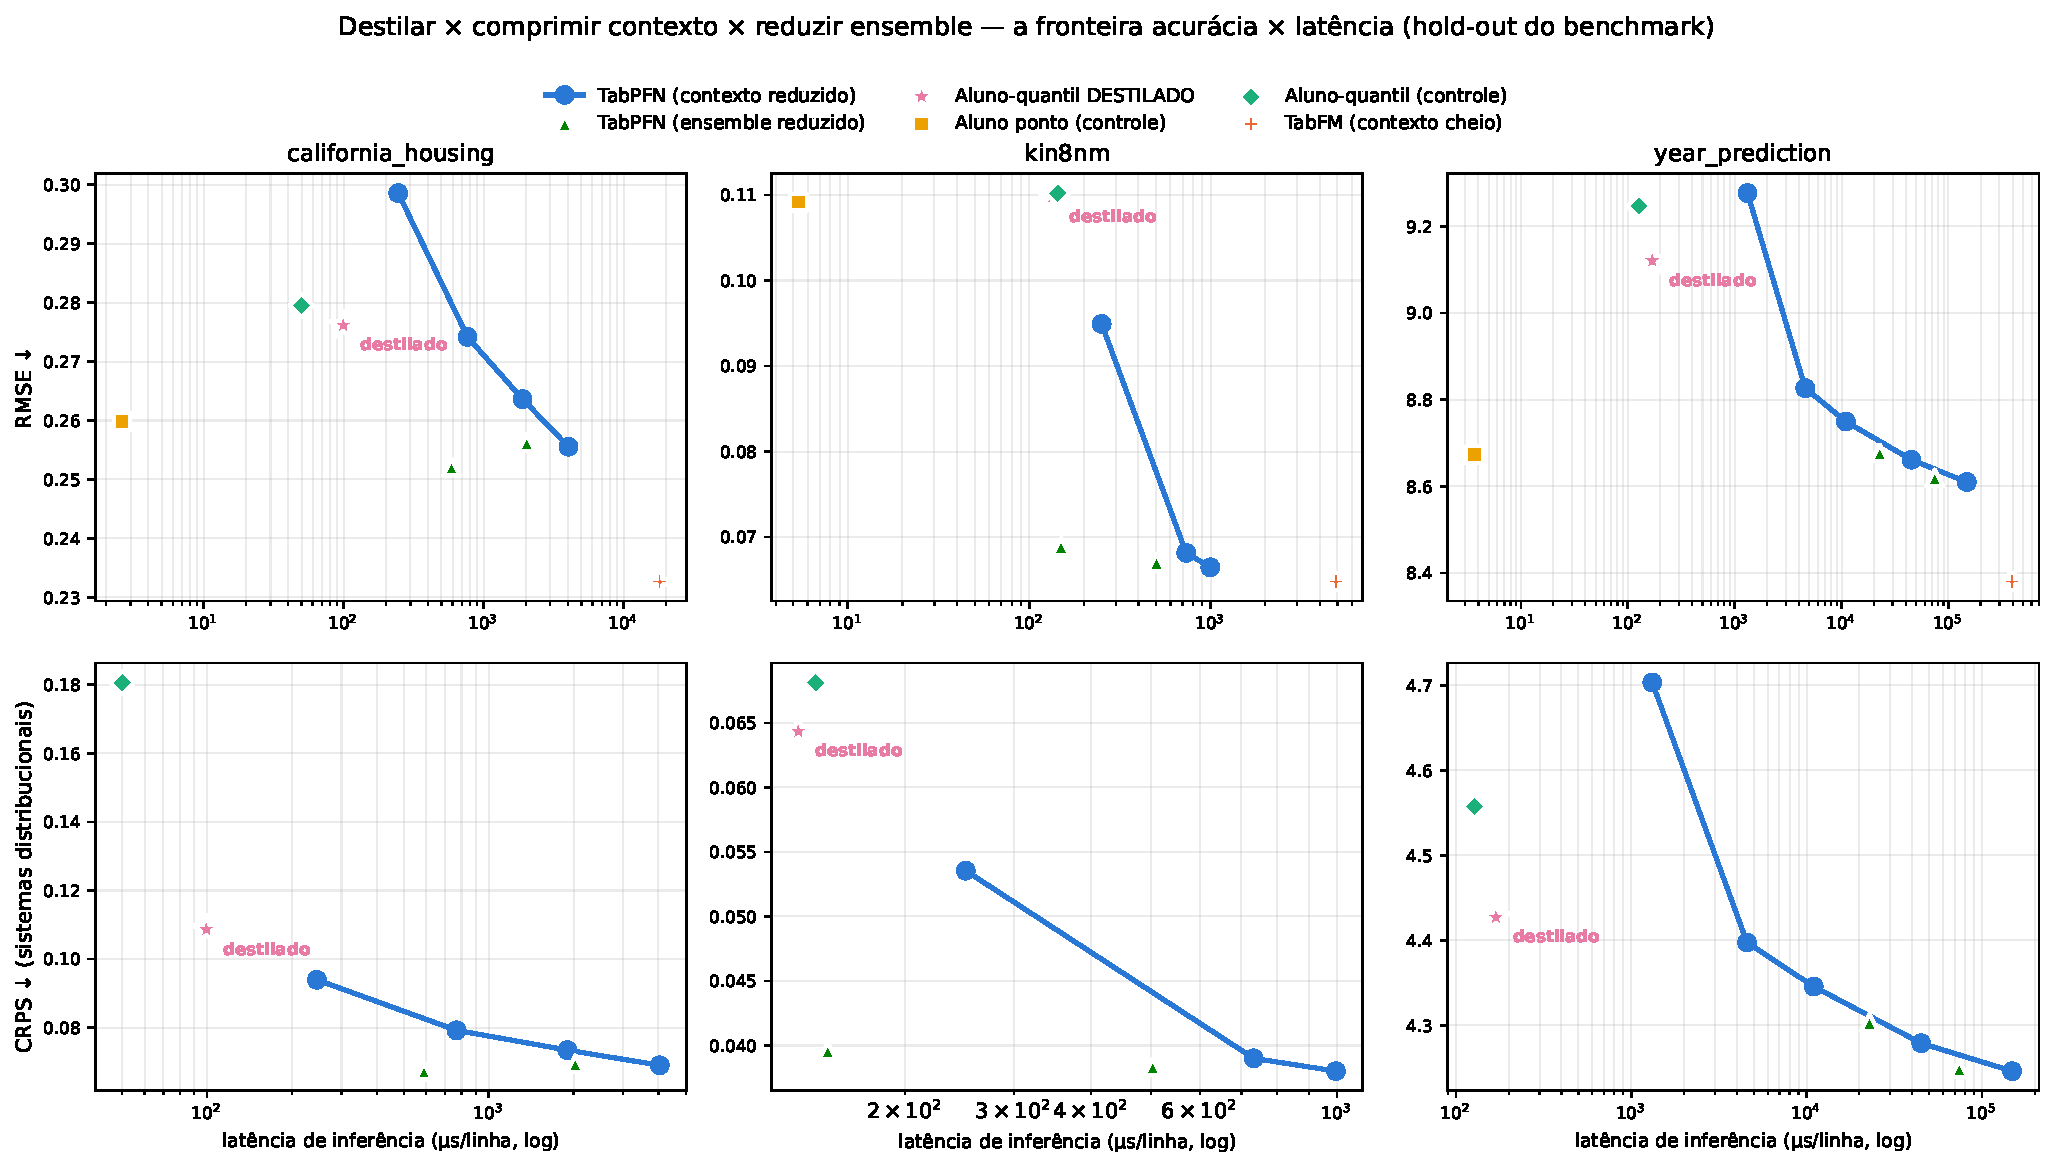
\includegraphics[width=\linewidth]{figures/pareto_distill.pdf}
\caption{The distill/compress/cache Pareto frontier on three positive-gap
datasets: CRPS (top) and RMSE (bottom) vs.\ serving latency (\us/row, log
scale). Below the sub-millisecond line the distilled multi-quantile student
is the only distributional option.
Source: \texttt{results/distillation/pareto.csv}.}
\label{fig:pareto}
\end{figure}

\subsection{Why out-of-fold labeling matters: calibration, not accuracy}
\label{sec:oof}

Classification results in prior work \citep{pocketfm2026} suggest in-sample
teacher labels collapse toward one-hot and must be avoided. Regression
behaves differently. Our three-regime ablation --- OOF (80\% context,
leak-free), in-sample at the \emph{same} 80\% context (leaky), and
in-sample at full context --- shows that leakage alone leaves RMSE and CRPS
intact (RMSE improves in all four datasets, CRPS in three), that context
size contributes little to accuracy (though on \texttt{wine\_quality} it
costs a further 5.9~p.p.\ of coverage), and that the harm is concentrated
in \textbf{coverage}: at identical context, in-sample-labeled students lose
0.5 to 5.1 points of PICP80 across all four datasets tested. The teacher is
overconfident on rows it has in context, and that overconfidence ---
invisible to accuracy metrics --- transfers to the student as too-narrow
intervals. OOF labeling in regression is therefore a calibration safeguard.
% results/distillation/ablation_insample.csv (3 regimes, 72 rows)

\begin{figure}[t]
\centering
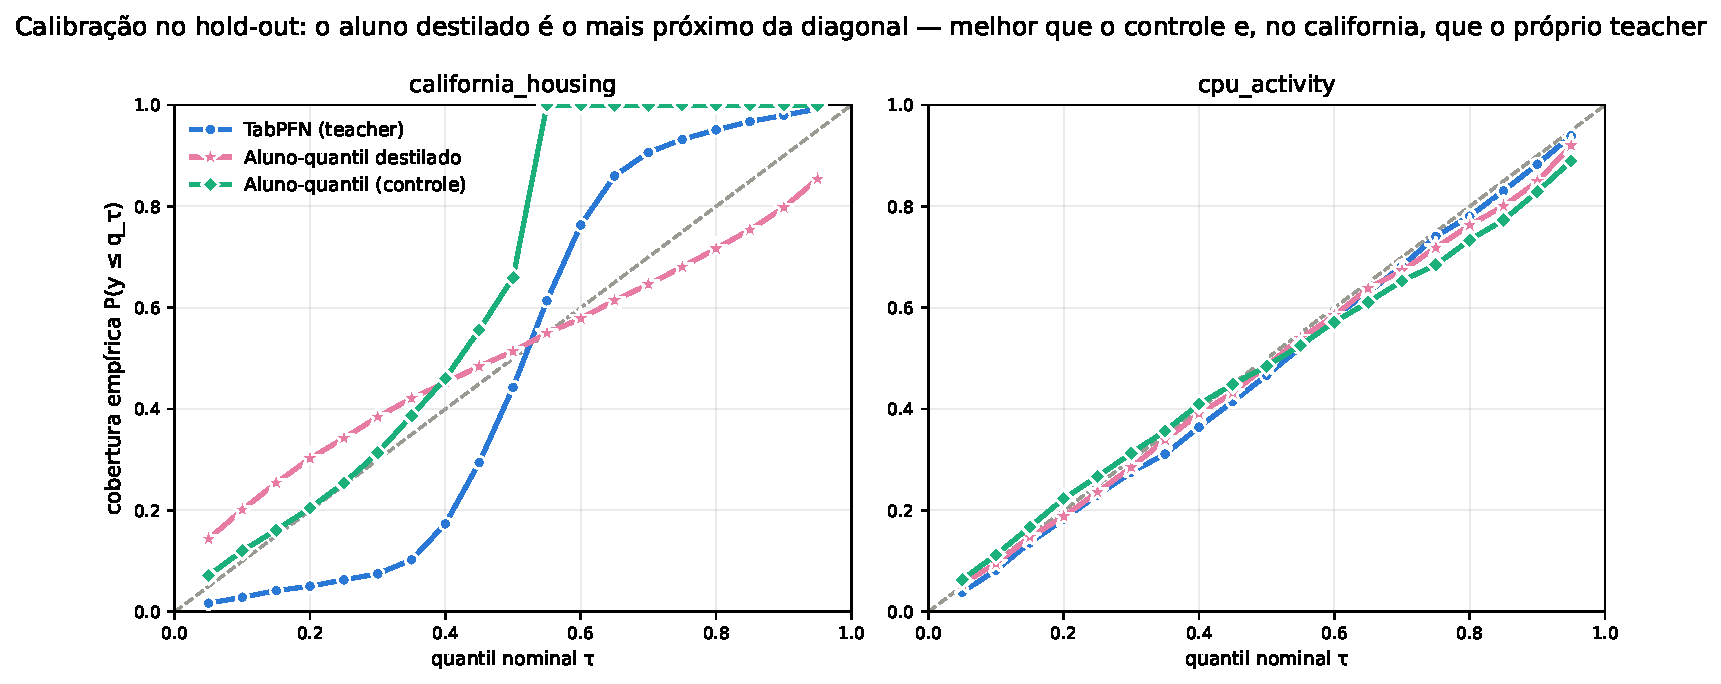
\includegraphics[width=\linewidth]{figures/calibration_distill.pdf}
\caption{Quantile reliability curves (empirical vs.\ nominal coverage per
$\tau$). The distilled student is closest to the diagonal on both panels;
on \texttt{california\_housing} it is better calibrated than the hard
control and than its own teacher.
Source: \texttt{results/figures/calibration\_distill.pdf} pipeline.}
\label{fig:calibration}
\end{figure}

\subsection{When to distill: two refuted hypotheses become a decision rule}
\label{sec:rule}

\emph{Does the student family matter?} Greatly. The XGBoost pinball
objective is a weak distributional learner, and distillation reliably
repairs it. A hard-label MLP-quantile student, by contrast, matches the
distilled XGBoost with no teacher at all on small numeric datasets (CRPS
0.110 vs.\ 0.109 on \texttt{california\_housing}; 0.047 vs.\ 0.064 on
\texttt{kin8nm}) --- yet collapses on \texttt{year\_prediction} (CRPS 9.66,
near-total overcoverage), where distillation rescues it ($\to$4.91).
% results/distillation/mlp_students.csv

\emph{Is heavy tail the failure moderator?} We re-ran teacher and students
under $y' = \log(1+y)$ on the three failing price-scale datasets plus two
positive controls. The transform does \textbf{not} rescue the failures
(\texttt{fifa} persists at $-1.69$) --- instead it collapses the teacher's
own edge (CRPS gaps shrink to 0.004--0.025 in log space) and shrinks the
successes too. Much of the TFM's distributional advantage on raw
price-scale targets \emph{is} scale handling, reproducible for free.
% results/distillation/ablation_logtarget.csv

Together these yield the paper's practical rule:

\begin{quote}
\textbf{Before distilling: (i) apply cheap target transforms; (ii) try a
strong native quantile student. Distill when a genuine teacher edge
persists after both --- one OOF labeling pass, costing minutes, measures
that edge directly.} Where the edge persists, distillation is the only
route to sub-millisecond distributional serving (\S\ref{sec:frontier}).
\end{quote}

\section{Discussion}

\paragraph{What distillation transfers.} Not the mean --- the \emph{shape}.
The consistent pattern across 20 datasets, two teachers, two student
families and three ablations is that point information saturates from raw
labels, while distributional information (quantile structure, calibrated
width) is teacher-borne and transferable --- exactly the component a
hard-label student cannot recover and the component priced most steeply by
in-context serving.

\paragraph{Point leader $\neq$ distributional leader.} TabFM leads every
accuracy table in the companion benchmark yet contributes nothing to the
distributional axis: its regression head is architecturally point-only, and
its ensemble spread is measurably useless as an uncertainty estimate
(16.3\% coverage at 80\% nominal). TabPFN's bar-distribution head emerges
as a genuine architectural moat, and our results argue that future TFMs
should ship distributional heads --- we quantify what their absence costs.

\paragraph{Serving guidance.} On 16\,GB-class hardware: reduce the ensemble
first (often free), compress context second, and reserve the full-context
teacher for accuracy-critical batch settings; when distributional
predictions must be served fast, the distilled quantile student is
currently the only occupant of that regime.

\section{Limitations}

Twenty datasets support significance at the 5\% level on both instruments,
but magnitudes remain heterogeneous (retention $-1.3$ to $+1.1$) and the
Bayesian posterior leaves ${\sim}25\%$ mass on negative retention --- the
decision rule of \S\ref{sec:rule}, not a universal claim, is the honest
deliverable. Students inherit benchmark-tuned capacity without per-target
re-tuning. CRPS is approximated on a 19-quantile grid. TabFM results refer
to the pinned v1.0.1 release, weeks old at the time of writing and without
a peer-reviewed reference. Single-GPU measurements bound, rather than
survey, the hardware space.

\section{Reproducibility}

All code, configs, seeds, per-experiment artifacts, the pre-registered
design with dated addenda, and two public corrections (a measurement-claim
retraction and a dataset-labeling erratum whose accidental duplicate run
reproduced the pipeline exactly) are in the public repository
(\url{https://github.com/Gvascons/master-thesis}). Weights of both teachers
are pinned; the 16\,GB VRAM ceilings and their mitigations are documented
as part of the method.

\section{Conclusion}

Tabular foundation models ended the accuracy tie; their serving cost is now
the binding constraint, and distillation attacks it selectively. In
regression, what survives the transfer is the distribution --- a median
19\% and up to the entirety of the teacher's CRPS edge at microsecond
latency --- under conditions a practitioner can verify in minutes. The rest
of the teacher's advantage either saturates from raw labels, dissolves
under a log transform, or waits on architectures that expose what their
training already knows.

\bibliographystyle{abbrvnat}
\bibliography{refs}

\end{document}
